\documentclass[9pt]{beamer}
\usetheme{Madrid}

% Update right margin since font size is now 9pt
\setbeamersize{text margin right=10mm} 

% Itemization settings
\usepackage{xpatch}
\xpatchcmd{\itemize}
  {\def\makelabel}
  {\ifnum\@itemdepth=1\relax
   \setlength\itemsep{2ex}% separation for first level
   \else
   \ifnum\@itemdepth=2\relax
     \setlength\itemsep{0.5ex}% separation for second level
   \else
     \ifnum\@itemdepth=3\relax
     \setlength\itemsep{0.5ex}% separation for third level
   \fi\fi\fi\def\makelabel
  }
 {}

\usepackage{bbold}
\usepackage{setspace}

\newcommand{\st}{s.t.\ }
\newcommand{\wrt}{w.r.t.\ }
\newcommand{\eg}{e.g.\ }
\newcommand{\eq}{\ =\ }
\newcommand{\andsp}{\text{ \ \ and \ \ }}

\usepackage{amsmath}
\usepackage{bm}
\newcommand{\bb}{\mathbb}
\newcommand{\mb}{\bm}
\newcommand{\mc}{\mathcal}

\usepackage{hyperref}
\hypersetup{
  colorlinks=false,
  linkcolor=blue,
  filecolor=blue,
  urlcolor=blue,
}

\title{On the Relationship between Self-Attention and Convolutional Layers}
\subtitle{Jean-Baptiste Cordonnier, Andreas Loukas, Martin Jaggi}
\author{Presented by Yenson Lau | Layer 6 AI}
\centering
\date{August 11th, 2021}

\begin{document}
\maketitle


\begin{frame}{Today's talk}
\begin{itemize} \setlength\itemsep{1em}
\item Attention can simultaneously attend to every word in an input sequence
\item NN architectures using self-attention (SA) only (without convolution) can compete with SA + convolutional architectures on vision tasks
\item Do SA layers process images in a similar manner to convolutional layers?
\end{itemize}
\end{frame}


\begin{frame}{Contributions of the paper}
\begin{itemize}
\item A constructive theoretical proof that SA can express convolutional layers using relative positional encoding:
\end{itemize}

\begin{center}
\vspace{.15in}
\noindent\fbox{
\parbox{0.85\textwidth}{
    \textbf{Main theorem.} \emph{A {\em multi-head self-attention} (MHSA) layer with $N_h$ heads of dimension $D_h$ each, final output dimension $D_{out}$, and a {\em relative positional encoding} of dimension $D_p\geq3$ can express any convolutional layer of kernel size $\sqrt{N_h}\times\sqrt{N_h}$ and $\min(D_h, D_{out})$ output channels.}
}}
\vspace{.2in}
\end{center}

\begin{itemize}
\item Experiments showing that the first few layers of DNNs using SA do behave similarly to the theoretical construction.
\end{itemize}
\end{frame}


\begin{frame}{Self-Attention}
\begin{itemize}
\item Let $\bm X\in\bb R^{T\times D_{in}}$ be an input matrix consisting of $T$ tokens in $D_{in}$ dimensions. A self-attention layer $\text{SA}:D_{in}\rightarrow D_{out}$ is expressed as
\begin{equation}
  \text{SA}(\mb X)_{t,:} \doteq \text{softmax}(\mb A_{t,:})\mb X\mb W_{val},
\end{equation}
\begin{center}
    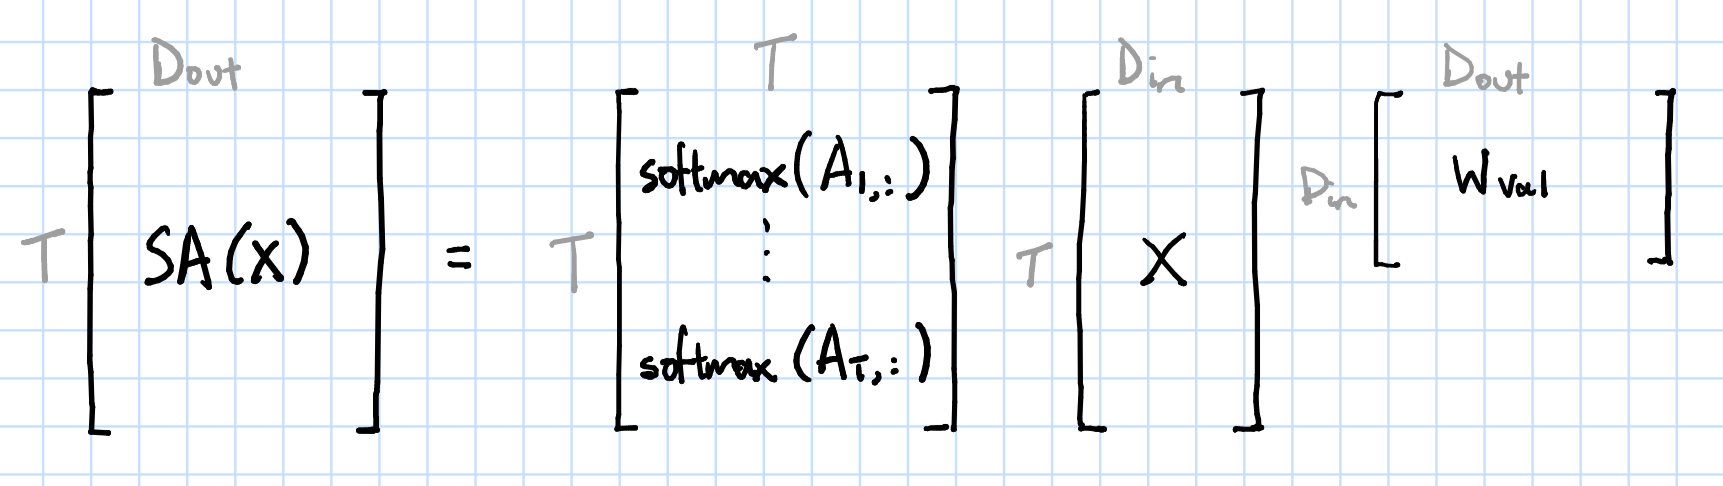
\includegraphics[width=.7\textwidth]{images/softmax.PNG}
\end{center}
\vspace{.1in}

\item We refer to the the elements of the $T\times T$ matrix
\begin{equation}
\mb A \doteq \mb X \mb W_{qry}\mb W_{key}^T\mb X^T
\end{equation}
the {\em attention scores}, and the softmax outputs as {\em attention probabilities}.
\end{itemize}
\end{frame}


\begin{frame}{Self-Attention}
\begin{itemize}
\item So far the learnable parameters are the {\em query}, {\em key}, and {\em value} matrices
$$\mb W_{qry} \in \bb R^{D_{in}\times{D_k}}, \ \ 
\mb W_{key} \in \bb R^{D_{in}\times{D_k}},\ \text{ and } \ 
\mb W_{val} \in \bb R^{D_{in}\times{D_{out}}}.$$
For simplicity, ignore residual connections, batch normalization or constant factors.

\vspace{.1in}
\item Note that $\bm A$ is {\em equivariant} -- shuffling the order of the tokens (rows) in $\bm X$ shuffles the token scores in $\bm A$. {\em This is not desired behavior.}
\begin{itemize}
    \item e.g. "the cat ate the fish" means something very different to "the fish ate the cat"
\end{itemize}

\vspace{.1in}
\item To overcome this, we can add a (fixed or learned) {\em positional encoding} $\bm P_{t,:}$, for each token in the sequence, to the input matrix for computing attention scores
\begin{equation}
A \doteq (\mb X + \mb P)\mb W_{qry}\mb W_{key}^T (\mb X + \mb P)^T,
\end{equation}
where the encoding matrix $\bm P$ has size $T\times D_{in}$.
\end{itemize}
\end{frame}


\begin{frame}{Multi-Head Self-Attention (MHSA)}
\begin{itemize}
\item In practice it is beneficial to replicate the SA mechanism into multiple heads, by concatenating the output of $N_h$ heads of output dimension $D_h$ and projecting it to dimension $D_{out}$.
\begin{equation}
\text{MHSA}(\mb X) \doteq \text{hcat}_{h\in[N_h]}\big[\text{SA}_h(\mb X)\big]\mb W_{out} + \mb b_{out}. \label{mhsa}
\end{equation}
Here $\bm W_{out}\in\bb R^{N_hD_h\times D_{out}}$ is the projection matrix and $\bm  b_{out}\in\bb R^{D_{out}}$ is a bias term.

\vspace{.2in}
\begin{center}
    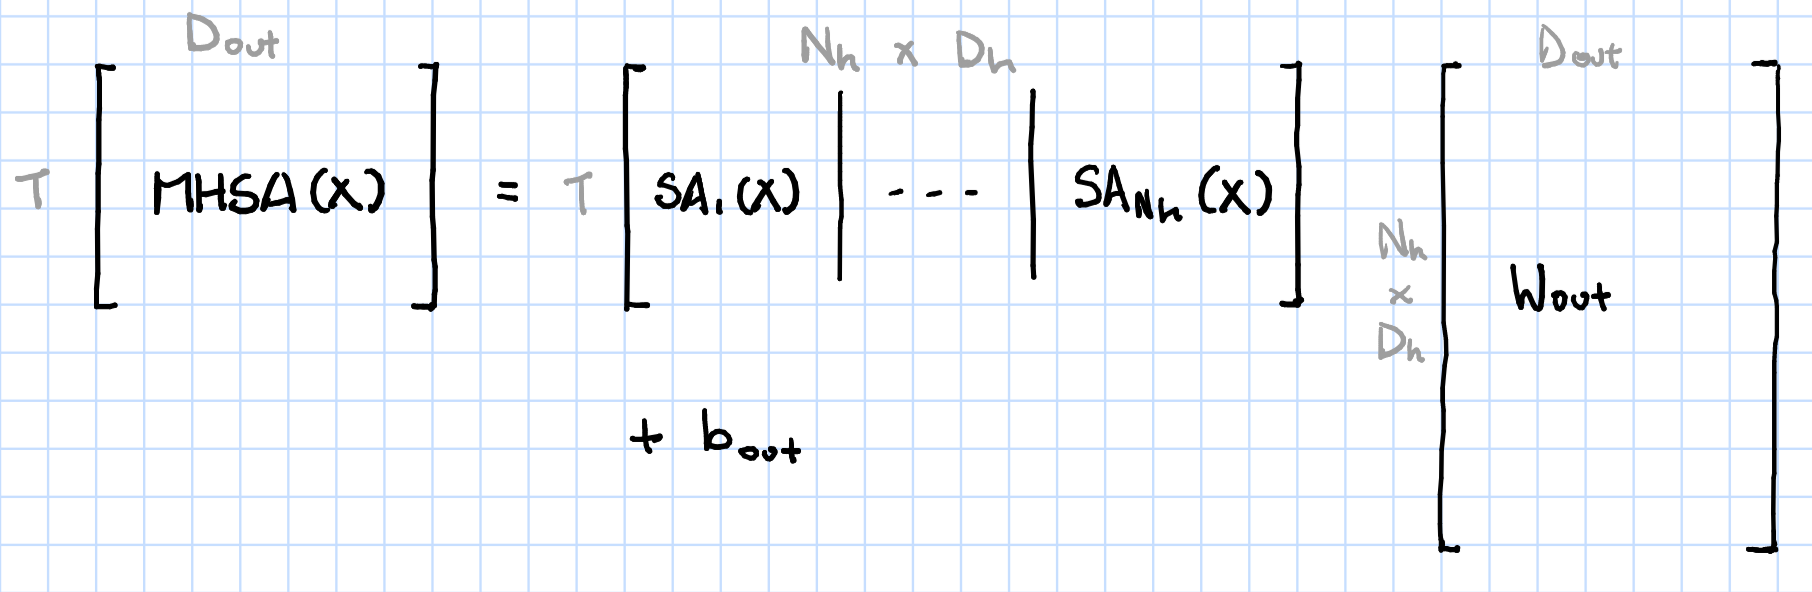
\includegraphics[width=.7\textwidth]{images/mhsa.PNG}
\end{center}
\end{itemize}
\end{frame}


\begin{frame}{Self-Attention for Images}
\begin{itemize}
\item Replace query and key tokens with pixels $\bm q, \bm k \in [W]\times[H]$, and the input with $\bm X \in \bb R^{W\times H\times D}$. Each attention score now associates a query and key pixel. 

\item For a pixel $\bm p\in (i,j), \bm X_{\bm p,:} \doteq \bm X_{i,j,:}$ and $\bm A_{\bm p, :} \doteq \bm A_{i,j,:,:}$. 

\item Then, analogously to the 1D case,
\begin{equation}
\text{Self-Attention}(\mb A)_{\mb q, :} \ = \ \sum_{\mb k} \text{softmax}(\mb A_{\mb q, :})_{\mb k}\ \mb X_{\mb k, :} \ \mb W_{val},
\end{equation}
and the MHSA retains the same form as Equation \eqref{mhsa}.
\end{itemize}
\end{frame}


\newcommand{\sqbrkt}[1]{\left[#1\right]}
\newcommand{\ktwo}{\left\lfloor\frac K2\right\rfloor}
\begin{frame}{Self-Attention for Images: Convolution}
\begin{itemize}
\item Given an image tensor $\bm X \in \bb R^{W\times H\times D_{in}}$ and kernel tensor $\bm W \in \bb R^{K\times K \times D_{in} \times D_{out}}$,
\begin{equation}
\text{Conv}(\mb X)_{i,j,:} \ \doteq \ \sum_{(\delta_1, \delta_2) \in \Delta_K} \mb X_{i-\delta_1, j-\delta_2, :} \mb W_{\delta_1, \delta_2, :, :} + \mb b \ \ \in \ \mathbb R^{D_{out}},
\end{equation}
where
$$\Delta_K \ \doteq \ \sqbrkt{-\ktwo, \dots, \ktwo} \times \sqbrkt{-\ktwo, \dots, \ktwo}$$
is the set of all shifts represented by a $K\times K$ kernel.

\vspace{.1in}
\item We depart from the original notation slightly by using the {\em unflipped} convolution. In the paper, the summand is flipped to $\bm X_{i+\delta_1, i+\delta_2,:} \bm W_{\delta_1, \delta_2,:,:}$. The theorem in the paper is not changed by this.
\end{itemize}
\end{frame}


\newcommand{\WW}{ \mb W_{qry}\mb W_{key}^T }
\begin{frame}{Relative Positional Encoding for Images}
\begin{itemize}
\item In {\em absolute encoding}, a fixed or learned vector $\bm P_{\bm p,:}$ is assigned to each pixel $\bm p$. 
\begin{align}
\mb A^{\text{abs}}_{\mb q, \mb k} 
\ &=\ (\mb X_{\mb q,:} + \mb P_{\mb q,:})\WW(\mb X_{\mb q,:} + \mb P_{\mb q,:})^T \nonumber
\\ &=\ \mb X_{\mb q,:}\WW\mb X^T_{k,:} +\ \mb X_{\mb q,:}\WW\mb P^T_{k,:} 
\\ &\qquad +\ \mb P_{\mb q,:}\WW\mb X^T_{k,:} \ +\ \mb P_{\mb q,:}\WW\mb P^T_{k,:}, \nonumber
\end{align}
where $\bm q$ and $\bm k$ correspond to the query and key pixels.

\vspace{.1in}
\item \emph{Relative positional encoding} instead considers the positional difference between the query pixel (pixel we compute the representation of) and the key pixel (pixel we attend to):
\begin{align}
\mb A^\text{rel}_{\mb q, \mb k} &= 
    \mb X_{\mb q,:}^T \WW \mb X_{k,:}
    + \mb X_{\mb q,:}^T \mb W_{qry}^T\hat{\mb W}_{key} \mb r_{\mb \delta}
    + \mb u^T \mb W_{key} \mb X^T_{k,:}
    + \mb v^T \hat{\mb W}_{key} \mb r_{\delta}.
\end{align}
\vspace{-.15in}
\begin{itemize}
    \item Learnable vectors $\bm u$, $\bm v$ are unique for each head 
    \item Relative positional encoding $\bm r_{\bm \delta} \in \bb R^{D_p}$ depends only on the shift $\bm \delta \doteq \bm k -\bm q$, and is shared by all layers and heads.
    \item Key weights are split into $\bm W_{key}$ for the input and $\hat{\bm W}_{key}$ for the positional encoding.
\end{itemize}

\end{itemize}
\end{frame}


\begin{frame}{Setup}
\begin{columns}
\begin{column}{0.6\textwidth}
  \begin{itemize}
    \item {\bf Two dates:} present ($t=0$) and future ($t=1$)
    \item World is fixed at $t=0$ but has $S$ states at $t=1$
    \begin{itemize}
      \item e.g. flipping a coin, prices go up or down, S=2
    \end{itemize}
    \vspace{1ex}

    \item $p_j$: \ price of a security $j$ at $t=0$
    \item $x^j_s$: \ payoff at $t=1$ for state $s$
    \vspace{2ex}

    \item Payoff vector for asset $j$
    \begin{align*}
      \bm x^j & \eq
      \begin{bmatrix}
        x^j_1 \\
        x^j_2 \\
        \vdots \\
        x^j_S
      \end{bmatrix}
      \ \in \bb R^S
    \end{align*}
  \end{itemize}
\end{column}

\begin{column}{0.38\textwidth} \centering
  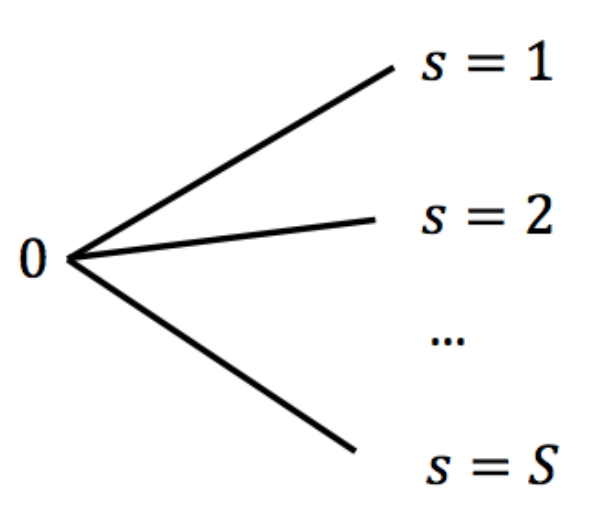
\includegraphics[width=.85\textwidth]{images/one-period.PNG}
\end{column}
\end{columns}
\end{frame}



\begin{frame}
\huge{Thanks!}
\end{frame}

\end{document}